\labeledsection{Deep Learning for NLP}{sec:dl}
\anondefinition{
A \defemph{word embedding} is a mapping from words in context into a real vector space $\mathbb{R}^n$ used for \linkterm{NLP}{NLP}
}{word_embedding}

\anondefinition{
A vector is called \defemph{one hot}, iff all its components are $0$ except for one $1$.
}{one_hot}

\anondefinition{
We call a \linkterm{word embedding}{word_embedding} \linkterm{one hot}{one_hot}, iff all of its vectors are.
}{one_hot_word_embedding}

\commandnote{
\linkterm{One hot word embeddings}{one_hot_word_embedding} are rarely used for actual tasks, but ofren used as a starting point for better \linkterm{word embeddings}{word_embedding}
}


\anondefinition{
Let $V = \set{t_1, \cdots, t_{\abs{V}}}$ be the vocabulary. The \defemph{one-hot embedding function} $E_{\text{hot}}: V \to \set{0,1}^{\abs{V}}$ maps each token $t_i$ to a vector $e_i$ where:
\[
e_{i, j} = 
\begin{cases} 
    1 & \text{if } i = j \\ 
    0 & \text{otherwise} 
\end{cases}
\]
}{one_hot_embedding_function}

\Example{
Let the vocabulary be $V = \set{\text{"apple"}, \text{"banana"}, \text{"cherry"}}$ with $\abs{V} = 3$, where $t_1 = \text{"apple"}$, $t_2 = \text{"banana"}$, and $t_3 = \text{"cherry"}$. 

Applying the \linkterm{one-hot embedding function}{one_hot_embedding_function} $E_{\text{hot}}: V \to \set{0,1}^3$ yields:
\[
E_{\text{hot}}(\text{"apple"}) = e_1 = \begin{pmatrix} 1 \\ 0 \\ 0 \end{pmatrix}, \quad
E_{\text{hot}}(\text{"banana"}) = e_2 = \begin{pmatrix} 0 \\ 1 \\ 0 \end{pmatrix}, \quad
E_{\text{hot}}(\text{"cherry"}) = e_3 = \begin{pmatrix} 0 \\ 0 \\ 1 \end{pmatrix}
\]
}{}


\observationbox{
Let $d = \tuple{t_1, \cdots, t_{\abs{d}}}$ be a document where $t_i \in V$. The \linkterm{word frequency vector}{BOW} $f_d \in \mathbb{N}^{\abs{V}}$ can be explicitly derived by summing the \linkterm{one hot word embeddings}{one_hot_word_embedding}:
\[
f_d = \sum_{i=1}^{\abs{d}} E_{\text{hot}}(t_i)
\]
}

\Example{
Following the previous example. If a document $d$ is given by the sequence of tokens $(\text{"banana"}, \text{"banana"}, \text{"apple"})$, the \linkterm{word frequency vector}{BOW} $f_d$ is induced by summing the individual \linkterm{one hot embeddings}{one_hot_word_embedding}:
\[
f_d = E_{\text{hot}}(\text{"banana"}) + E_{\text{hot}}(\text{"banana"}) + E_{\text{hot}}(\text{"apple"}) = \begin{pmatrix} 0 \\ 1 \\ 0 \end{pmatrix} + \begin{pmatrix} 0 \\ 1 \\ 0 \end{pmatrix} + \begin{pmatrix} 1 \\ 0 \\ 0 \end{pmatrix} = \begin{pmatrix} 1 \\ 2 \\ 0 \end{pmatrix}
\]
}{}


\anondefinition{
The \defemph{softmax} function $\sigma: \mathbb{R} \times \mathbb{R}^k \to \mathbb{R}^k$ is defined by:
\[
\sigma_{\beta}(z)_i := \frac{e^{\beta z_i}}{\sum_{j=1}^{k}e^{\beta z_j}}
\]

where $z = \tuple{z_1, \cdots, z_k}$, $i \in \set{1, \cdots k}$. We call $e^{\beta}$ the \defemph{base} of $\sigma$. For $\beta = 1$, we call $\sigma$ the \defemph{standard softmax} function.
}{softmax}

\Example{
Let $z = \tuple{1.0, 2.0, 3.0}$ be a vector in $\mathbb{R}^3$ (so $k = 3$), where $z_1 = 1.0$, $z_2 = 2.0$, and $z_3 = 3.0$. 

\begin{enumerate}
    \item \textbf{Standard Softmax ($\beta = 1$):}
    First, compute the exponentials for the denominator:
    \[
    e^{1 \cdot 1.0} \approx 2.718, \quad e^{1 \cdot 2.0} \approx 7.389, \quad e^{1 \cdot 3.0} \approx 20.086
    \]
    The sum of these values is $\sum_{j=1}^{3} e^{z_j} \approx 2.718 + 7.389 + 20.086 = 30.193$. 
    
    Applying the function component-wise yields:
    \[
    \sigma_{1}(z) \approx \tuple{\frac{2.718}{30.193}, \frac{7.389}{30.193}, \frac{20.086}{30.193}} \approx \tuple{0.090, 0.245, 0.665}
    \]

    \item \textbf{Softmax with a different base ($\beta = 0.5$):}
    Compute the scaled exponentials:
    \[
    e^{0.5 \cdot 1.0} \approx 1.649, \quad e^{0.5 \cdot 2.0} \approx 2.718, \quad e^{0.5 \cdot 3.0} \approx 4.482
    \]
    The new sum is $\sum_{j=1}^{3} e^{0.5 z_j} \approx 1.649 + 2.718 + 4.482 = 8.849$.
    
    Applying the function yields a smoother probability distribution:
    \[
    \sigma_{0.5}(z) \approx \tuple{\frac{1.649}{8.849}, \frac{2.718}{8.849}, \frac{4.482}{8.849}} \approx \tuple{0.186, 0.307, 0.507}
    \]
\end{enumerate}
}{}

\problembox{
\begin{itemize}
    \item Those \linkterm{one hot word embeddings}{one_hot_word_embedding} do not capture meaning / semantics
    \item For large vocabulary size, \linkterm{one hot word embeddings}{one_hot_word_embedding} become intractable
\end{itemize}
}

\questionbox{
Can we represent words in vectors so the actual meaning is captured and we have size much less than $\abs{V}$? 
}

\ideabox{
We want \linkterm{word embeddings}{word_embedding} that captures the word meanings, e.g. the \linkterm{embedding}{word_embedding} of "apple", "banana", etc... should have high \linkterm{cosine similarity}{cosine_similarity}.
}


\answerbox{
Yes. That's when the \textbf{word2vec} project started!
}

\anondefinition{
\defemph{Word2vec} is a system designed to solve one specific problem: How do we turn human words into a geometric map of coordinates so a computer can understand meaning?
}{word2vec}


\observationbox{
To build this semantic map, Word2Vec forces the computer to play a predictive guessing game over millions of sentences. Instead of analyzing text globally, it slides a small window across a sentence, isolates a specific word, and looks at its immediate neighbors (the \defemph{context}).
}

\questionbox{
How can a computer play a guessing game using words if it only understands numbers?
}

\answerbox{
We use the \linkterm{one-hot embedding function}{one_hot_embedding_function}. Before a sentence hits the predictive system, an automated translator converts every human word into its unique, rigid one-hot vector based on the vocabulary $V$. 

For example, given the sentence \textit{"The monkey ate a banana"}, the system converts it into \linkterm{one hot word embeddings}{one_hot_word_embedding}:
\[
e_{\text{"the"}}, \quad e_{\text{"monkey"}}, \quad e_{\text{"ate"}}, \quad e_{\text{"a"}}, \quad e_{\text{"banana"}}
\]
}

\questionbox{
What is the system that takes these vectors and actually makes the guess?
}

\answerbox{
We feed these vectors into a simple, single-\linkterm{layer}{layers_neural_nets} \linkterm{Neural Network}{ann}.
}

\anondefinition{
The \defemph{Continuous Bag-of-Words (CBOW)} algorithm is one of the foundational architectures inside the \linkterm{word2vec}{word2vec} framework. In the CBOW setup over a vocabulary $V$, we hide a single target word from the network and feed it the sparse \linkterm{one-hot vectors}{one_hot_word_embedding} in $\set{0,1}^{\abs{V}}$ of the surrounding context words. The network compresses these inputs into a dense hidden layer of dimension $d$, where $d \ll \abs{V}$, and uses this bottleneck state to predict the \linkterm{one-hot vector}{one_hot_word_embedding} of the missing target word.
}{CBOW}

\Example{
Suppose we use a context window of size $C=2$ on the sentence:
\[
\text{"The monkey ate a banana today."}
\]
If our target word is $t=$ \textit{"banana"}, the algorithm hides it and extracts the surrounding context words within the window:
\[
\text{Context} = \set{\text{"ate"}, \text{"a"}, \text{"today"}}
\]
The network is fed the one-hot vectors for \textit{"ate"}, \textit{"a"}, and \textit{"today"}, and its objective is to output a probability distribution via the \linkterm{standard softmax}{softmax} function that perfectly matches the true one-hot target vector:
\[
e_{\text{"banana"}} = \begin{pmatrix} 0 \\ \vdots \\ 1 \\ \vdots \\ 0 \end{pmatrix}
\]
}{}

\begin{figure}[H]
    \centering
    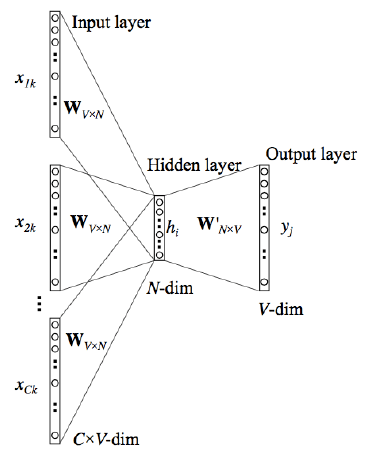
\includegraphics[width=0.3\linewidth]{images/CBOW.png}
\end{figure}

\observationbox{
\begin{itemize}
    \item Using e.g. \linkterm{cosine similarity}{cosine_similarity} to compare vectors, we can find words with similar meanings.
    \item Semantic and syntactic relationships emerge as arithmetic relations
\end{itemize}
}

\begin{figure}[H]
    \centering
    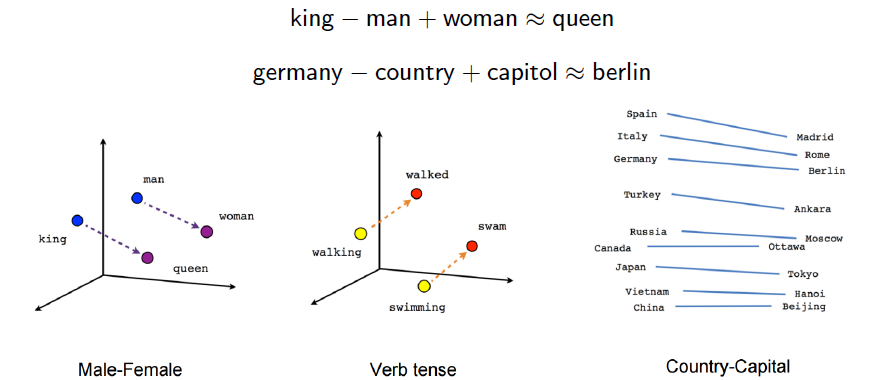
\includegraphics[width=0.6\linewidth]{images/semantics_CBOW.png}
\end{figure}

\anondefinition{
A \linkterm{Neural Network}{ann} is called \defemph{recurrent} (an \defemph{RNN}), iff it has \linkterm{cycles}{cyclic_graphs}
}{RNN}

\Example{
\textbf{A simple \linkterm{RNN}{RNN}}

It has an \linkterm{input layer}{layers_neural_nets} $x$, a \linkterm{hidden layer}{layers_neural_nets} $z$ with recurrent connections and delay $\Delta$, and an \linkterm{output layer}{layers_neural_nets} $y$:

\begin{figure}[H]
    \centering
    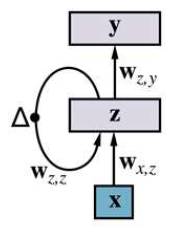
\includegraphics[width=0.1\linewidth]{images/simple_RNN.png}
\end{figure}

For a time step $t$, we have:
\begin{align*}
    z_t &= g_z(W_{z,z} z_{t-1} + W_{x,z} x_t) \\ 
    y_t &= g_y(W_{z,y}z_t)
\end{align*}

where $g_z$ and $g_y$ are the \linkterm{activation functions}{ann} for the \linkterm{hidden}{layers_neural_nets} and \linkterm{output}{layers_neural_nets} \linkterm{layers}{layers_neural_nets}.
}{ex:simple_RNN}

\ideabox{
For training, unroll the \linkterm{RNN}{RNN} into a \linkterm{Feed-Forward Neural Network}{ffnn} $\leadsto$ \linkterm{Backpropagation}{backpropagation}
}

\Example{
The \linkterm{RNN}{RNN} from \exampleref{ex:simple_RNN} unrolled three times:

\begin{figure}[H]
    \centering
    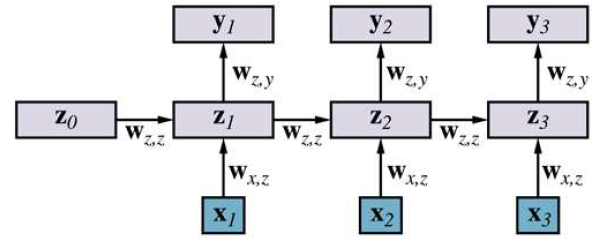
\includegraphics[width=0.4\linewidth]{images/simple_RNN_unrolled.png}
\end{figure}
}{}

\anondefinition{
The \defemph{Back-Propagation Through Time (BPTT)} algorithm carefully maintains the identity of $W_{z,z}$ over all steps.
}{BPTT}

\observationbox{
\linkterm{RNN}{RNN} do not have a fixed length input
}

\problembox{
\linkterm{RNN}{RNN} accepts input (e.g. words) in certain order (left-to-right), i.e. at any particular time step $t$ we only look at the words that came before. 
}

\redbox{
Sometimes, we want context from both left and right!
}

\Example{
\begin{itemize}
    \item \textit{Eduardo told me that Miguel was very sick, so I took him to the hospital}
    \item \textit{Eduardo told me that Miguel was very sick, so I took him to see Miguel}
\end{itemize}

\textit{him} in the first sentence refers to \textit{Miguel} but in the second refers to \textit{Eduardo}. We infered that based on the "right context"
}{}

\anondefinition{
A \defemph{Bidirectional RNN (BRNN)} concatenates a right-to-left model onto a left-to-right model.
}{BRNN}

\Example{
\linkterm{BRNN}{BRNN} for \linkterm{POS tagging}{POS_tagging}:
\begin{figure}[H]
    \centering
    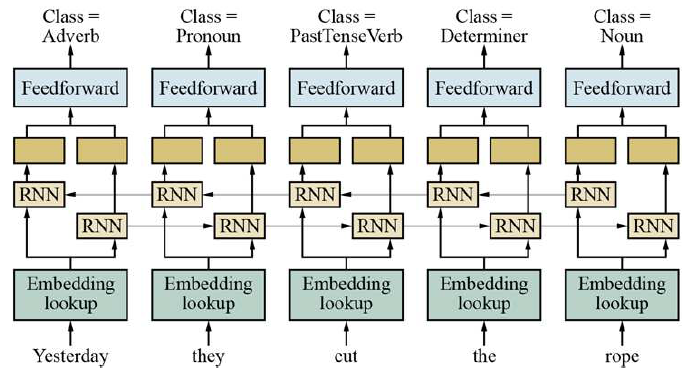
\includegraphics[width=0.4\linewidth]{images/BRNN.png}
\end{figure}
}{}

\problembox{
When training a vanilla \linkterm{RNN}{RNN} using \linkterm{BPTT}{BPTT}, the long-term gradients which are back-propagated can "vanish" (tend to zero) ot "explode" (tend to infinity)
}

\anondefinition{
\defemph{Long Short-Term Memory (LSTM)} provides a short-term memory for \linkterm{RNN}{RNN} that can last thousands of time steps.
}{LSTM}

\commandnote{
An \linkterm{LSTM}{LSTM} can learn when to remember and when to forget information
}

\titledbox{LSTM Idea}{
\begin{itemize}
    \item Instead of taking the output of the \linkterm{RNN}{RNN} directly, we introduce an additional memory vector $c$ (initially copied from the previous time step)
    \item The recurrent (short-term memory) vector $z$ is also there 
    \item We introduce three "gates":
    \begin{enumerate}
        \item forget gate $f$
        \item input gate $i$
        \item output gate $o$
    \end{enumerate}
    \item The forget gate gets trained to decide which component of the vector $c$ we retain or forget
    \item The input gate decides which components of the current input to \textbf{add} to $c$
    \item The output gate decides which components of $c$ to output as $z$
\end{itemize}
}

\observationbox{
The \textbf{addition} trick is what tackles the vanishing gradient problem
}